\documentclass[a4paper,12pt]{article}
\usepackage[utf8]{inputenc}
\usepackage[spanish]{babel}
\usepackage{hyperref}
\usepackage{geometry}
\usepackage{graphicx}
% Configuración de márgenes
\geometry{left=2.5cm,right=2.5cm,top=3cm,bottom=3cm}

% Configuración del enlace clicable
\hypersetup{
    colorlinks=true,
    linkcolor=blue,
    urlcolor=blue,
    pdftitle={Implementación del Juego 3 en Raya},
    pdfauthor={Adrián Martínez Pérez, Guillem Arnau Vallejos}
}

% Información del documento
\title{Implementación del Juego 3 en Raya}
\author{Adrián Martínez Pérez \\ Guillem Arnau Vallejos}
\date{Facultad de Informática de Barcelona \\ Grado de Inteligencia Artificial}

\begin{document}

\maketitle
\tableofcontents
\newpage

\section{Introducción}
El objetivo de esta práctica es implementar un tablero abstracto para el juego 3 en raya, utilizando el módulo
\texttt{pygame} de \texttt{python3}. Inicialmente, en esta primera versión, hemos desarrollado el juego para ser
 jugado por dos personas, en lugar de incluir una inteligencia artificial que permita competir contra la máquina,
 decisión la cual nos ha permitido enfocarnos en el desarrollo de la lógica del juego y en la creación de una buena 
 experiencia de usuario funcional y accesible.

 \vspace{\baselineskip}
 También hemos hecho accesible el código para todo aquel que quiera leerlo, entenderlo o modificarlo, ya que está todo
 comentado en la medida de lo posible, tanto lo que hacen las funciones, como las diferentes partes de ellas. 
 Además, todo el juego ha sido desarrollado para que pueda ser cambiado el tamaño del teablero y las piedras por jugador,
 simplemente cambiando el valor de \texttt{BSIZ} y \texttt{ST\_PLAYER} en el archivo \texttt{constants.py}, manteniendo una 
 dinámica más entretenida se pretende jugar con un tablero más grande para hacer el juego más largo (y más complicado).

 \vspace{\baselineskip}
 El juego consta de cinco archivos principales que estructuran el código 
 y separan las funcionalidades esenciales:

 \begin{itemize}
    \item \textbf{\texttt{abs\_board\_h.py}}: Funciones y lógica necesarias para gestionar el estado del tablero,
    verificar condiciones de victoria y manejar los movimientos de los jugadores.
    \item \textbf{\texttt{constants.py}}: Este archivo sirve para almacenar todas las constantes necesarias para el
    funcionamiento del programa.
    \item \textbf{\texttt{utils.py}}: Implementa las utilidades del juego: tanto las pantallas de carga en el modo texto
    (\texttt{txt}) como en la interfaz gráfica (\texttt{gui}), y el menú principal.
    \item \textbf{\texttt{main\_gui.py}}: Implementa la interfaz gráfica de usuario. Contiene la configuración inicial,
    creación de ventanas e integración con \texttt{abs\_board\_h.py}.
    \item \textbf{\texttt{main\_txt.py}}: Implementa la versión para consola del juego, con colores y mejoras visuales
    para un mayor atractivo.
\end{itemize}

En la carpeta de la práctica se incluye todo lo necesario para la ejecución y disfrute del juego. Solo es necesario
ejecutar dos archivos para jugar al juego:

\begin{itemize}
    \item Para jugar en modo texto, ejecutar en la consola el siguiente comando:
    \begin{verbatim}
    $ python3 main_txt.py
    \end{verbatim}
    \item Para jugar en modo gráfico, ejecutar en la consola el siguiente comando:
    \begin{verbatim}
    $ python3 main_gui.py
    \end{verbatim}
\end{itemize}

\section{Metodología de la Implementación}
El desarrollo de este proyecto ha sido un trabajo colaborativo entre Adrián Martínez Pérez y Guillem Arnau Vallejos,
mediante un repositorio compartido en la plataforma \texttt{GitHub}. Esta plataforma nos permitió realizar un seguimiento
de los cambios, revertir errores y garantizar la estabilidad del código en cada etapa del desarrollo. GitHub ha sido una 
excelente plataforma para la colaboración en este tipo de proyectos, y hemos disfrutado mucho aprendiendo a utilizarla.

\vspace{\baselineskip}
En cuanto a la distribución de tareas, adoptamos un enfoque flexible. No dividimos las tareas de manera estricta, sino que
trabajamos de forma iterativa comunicándonos constantemente sobre los avances, problemas encontrados, mejoras implementadas y 
las ideas para futuras versiones. Esta dinámica fomentó un ambiente de aprendizaje mutuo y creatividad.

\vspace{\baselineskip}
Para la implementación de este código, hemos añadido un archivo que no estaba originalmente: \texttt{utils.py}, y hemos
modificado todos los archivos con el fin de lograr una buena implementación, teniendo creatividad además de añadir nuevas
funciones y utilidades, como una animación de carga para el modo de juego txt.

\section{Explicación del Código}
Para poder explicar todo el código sobre como funciona nuestra implementación del juego del tres en raya, debemos de explicar
todos los archivos que hemos modificado \texttt{abs\_board\_h.py, constants.py, main\_gui.py y main\_txt.py}, además del archivo 
de nueva creación que hemos incluido nosotros: \texttt{utils.py}.

\subsection{abs\_board\_h.py}
Inicialmente, en este archivo solo se nos dierno nombradas las funciones que debíamos de utilizar, dejándonos a nosotros una libre 
implementación del código. La función principal es set\_board\_up, la cual inicializa el tablero, y dentro de esta función tenemos la
lógica de todo el tablero. Modificamos todas y cada una de las funciones para implementar la lógica del juego, y hacer que fuera sencillo 
de entender.

\vspace{\baselineskip}
En este archivo se inicializan todas las variables necesarias, como el tablero (con medida \textit{BSIZ}, definida en constants.py,
y que permite que se pueda cambiar el tamaño del tablero), las piedras jugadas y las no jugadas en forma de una lista, el jugador
actual al que le tocaría mover piedra, y la piedra seleccionada en el turno actual.
A continuación, se explican cada una de ellas:

\begin{itemize}
    \item \texttt{stones}: Retorna un iterador sobre las piedras que ya se han colocado en el tablero.
    \item \texttt{select\_st}: Selecciona una piedra del tablero para moverla, y toma como parámetros \textit{i} y \textit{j}, las
    cuales son las coordenadas de la piedra a seleccionar, y retorna True si la selección es exitosa, o False si la selección no es 
    válida.
    \item \texttt{end}: Comprueba las condiciones de victoria y muestra el ganador. Además, esta función es clave para el funcionamiento
    del modo de juego \textit{misery}, ya que incluye una comprobación para el modo de juego, el cual invierte al ganador.
    \item \texttt{move\_st}: Coloca una nueva piedra en el tablero, hasta que se acaban, y entonces cambia su comportamiento para mover la 
    piedra seleccionada. Al igual que la anterior, recibe las coordenadas de la piedra. Esta función retorna una tupla que indica si el movimiento
    fue válido, el jugador actual y si el juego ha terminado.
    \item \texttt{draw\_txt}: Dibuja el estado actual del tablero cuando está seleccionado el modo txt, y hemos realizado mejoras visuales para que 
    el tablero se vea atractivo con el uso de símbolos ASCII.\@
\end{itemize}

\vspace{\baselineskip}
\subsection{constants.py}
Dentro de este archivo se definen todas las constantes del juego, haciéndolo así más modificable. Incluye el tamaño del tablero, las piedras por jugador,
los colores del juego para el modo gui, además del tamaño de la ventana, celdas vacías, tamaño de las piedras\ldots
Además, nos sentimos libres de añadir un nuevo diccionario llamado \texttt{COLORES}, dentro del cual se definen nuevos colores como el amarillo, violeta,
magenta o cyan. Todo esto con el fin de modificar los colores en el modo txt, que se impriman las fichas con diferentes colores, o incluso la animación de carga.
Gracias a este diccionario, se pueden modificar los colores fácilmente, y son accesibles para todos los archivos python, e incluso podríamos añadir colores
a los logs de cada archivo para detectar posibles fallos más fácilmente.

Pensamos en utilizar en este código el formato de secuencia de escape ANSI, ya que con esta codificación es más fácil modificar el texto, como podría ser ponerlo
en negrita o cursiva, en lugar del formato tradicional RGB. 

\subsection{utils.py}
Este archivo no estaba inicialmente en el código proporcionado, pero lo hemos considerado muy útil para implementar diversas funcionalidades, como el menu de inicio o 
las pantallas de los ganadores.

\vspace{\baselineskip}
Primeramente, la primera función en este archivo es \texttt{draw\_winner\_board}, la cual implementa la pantalla del ganador del juego. Esta función acepta como parámetro 
a \textit{winner}, el cual es el ganador del juego. Primeramente incluye una comprobación para verificar el archivo que ha sido ejecutado (main\_gui.py o main\_txt.py), con el 
objetivo de mostrar una interfaz u otra. En este caso, si el modo de juego seleccionado es txt, se llama a la función \texttt{draw\_winner\_txt} la cual es la encargada de 
dibujar el ganador en el modo txt, y se le pasa el parámetro winner.

\vspace{\baselineskip}
Esta función renderiza una nueva ventana utilizando el módulo \texttt{pygame}, y se encarga de renderizar un texto u otro en base al ganador (pasado como winner a la función), y 
dependiendo del modo de juego.

\vspace{\baselineskip}
Posteriormente, hemos implementado la función \texttt{draw\_winner\_txt}, la cual se encarga de dibujar la pantalla del ganador en el modo txt. Esta función recive como parámetro 
el ganador del juego, y se imprime el texto en consola en diferentes colores utilizando el diccionario anteriormente mencionado para un mayor atractivo visual.

\vspace{\baselineskip}
La última función en este archivo es \texttt{show\_menu}, la cual fue todo un reto de programación. Esta función implementa el menú
principal del juego, y por ello es una de las más importantes.

\vspace{\baselineskip}
Dibuja una ventana con el título del juego, y con la posibilidad de seleccionar el modo de juego 'Normal' o 'Misery', con dos atractivos 
botones rojos y con un hover azul, el cual se muestra al pasar el ratón por encima. Debajo se muestran los autores del juego.
\begin{figure}[htbp]
    \centering
    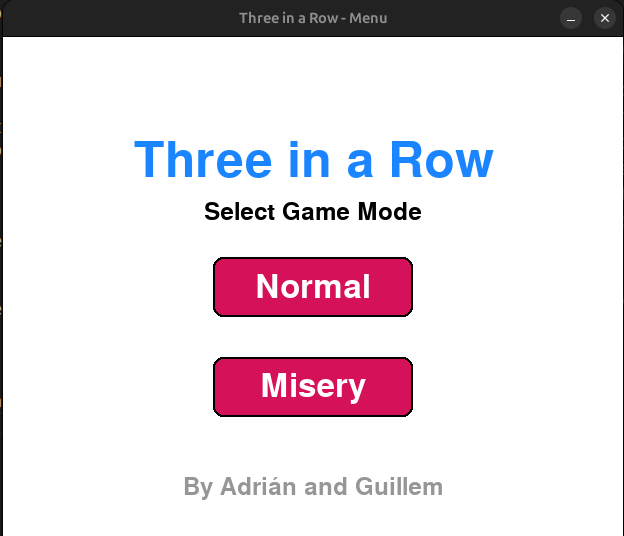
\includegraphics[width=0.8\textwidth]{./imagenes/menu_inicio.png}
    \caption{Menú principal del juego en el modo gui.}
    \label{fig:etiqueta}
\end{figure}

\end{document}
